\section{Laboratory work implementation}

\subsection{Tasks and Points}

\begin{enumerate}

\item Draw 5 lines of different colors and weights
\item Draw 2 Bezier curves
\item Draw 4 plane objects (circle, oval, rectangle, square) of different colors, weights, filled and not
\item Draw 2 different objects using mouse
\item Draw a custom bitmap image
\item Fill 2 object with gradient
\item Hook keyboard input. Add 2 different keyboard combinations that will change mouse ability to draw objects
\item Draw a Bezier curve using mouse
\item Use mouse as an eraser with adjustable width

\end{enumerate}
\subsection{Laboratory work analysis}

Link to my GitHub repository : 

\url{https://github.com/Tolea86/WP_ANDROID/tree/master/LAB_3/PW_LAB3}\\

My application has following features : it has 3 main views, first Main View is the basic view, which contains 5 lines of different colors and weights and positioned differently, 2 Bezier curves, 4 plane objects (circle, oval, square and rectangle), and a button "Next Part" which directs to the next part of the app. The next view is Normal View with 2 objects first without a gradient and 4 buttons, Draw Bitmap, Hook Keyboard, Previous Part and Next Part. Previous Part button directs to Basic Activity, Next Part to Advanced Activity. Clicking on Draw Bitmap will draw the Bitmap of the current screen as if making screen shot by drawing it pixel by pixel. Clicking on Hook Keyboard will open the keyboard. Clicking the button "C" (from circle) will make the circle from the view appear with gradient. Clicking the button "R" will make the rectangle from the view appear with gradient. In Advanced Activity we have 5 buttons. One setting the mouse to brush, other to eraser, 3 buttons to control the size of the brush. And white square at the bottom is our draw section.

\subsection{Prove your work with screens}

a)

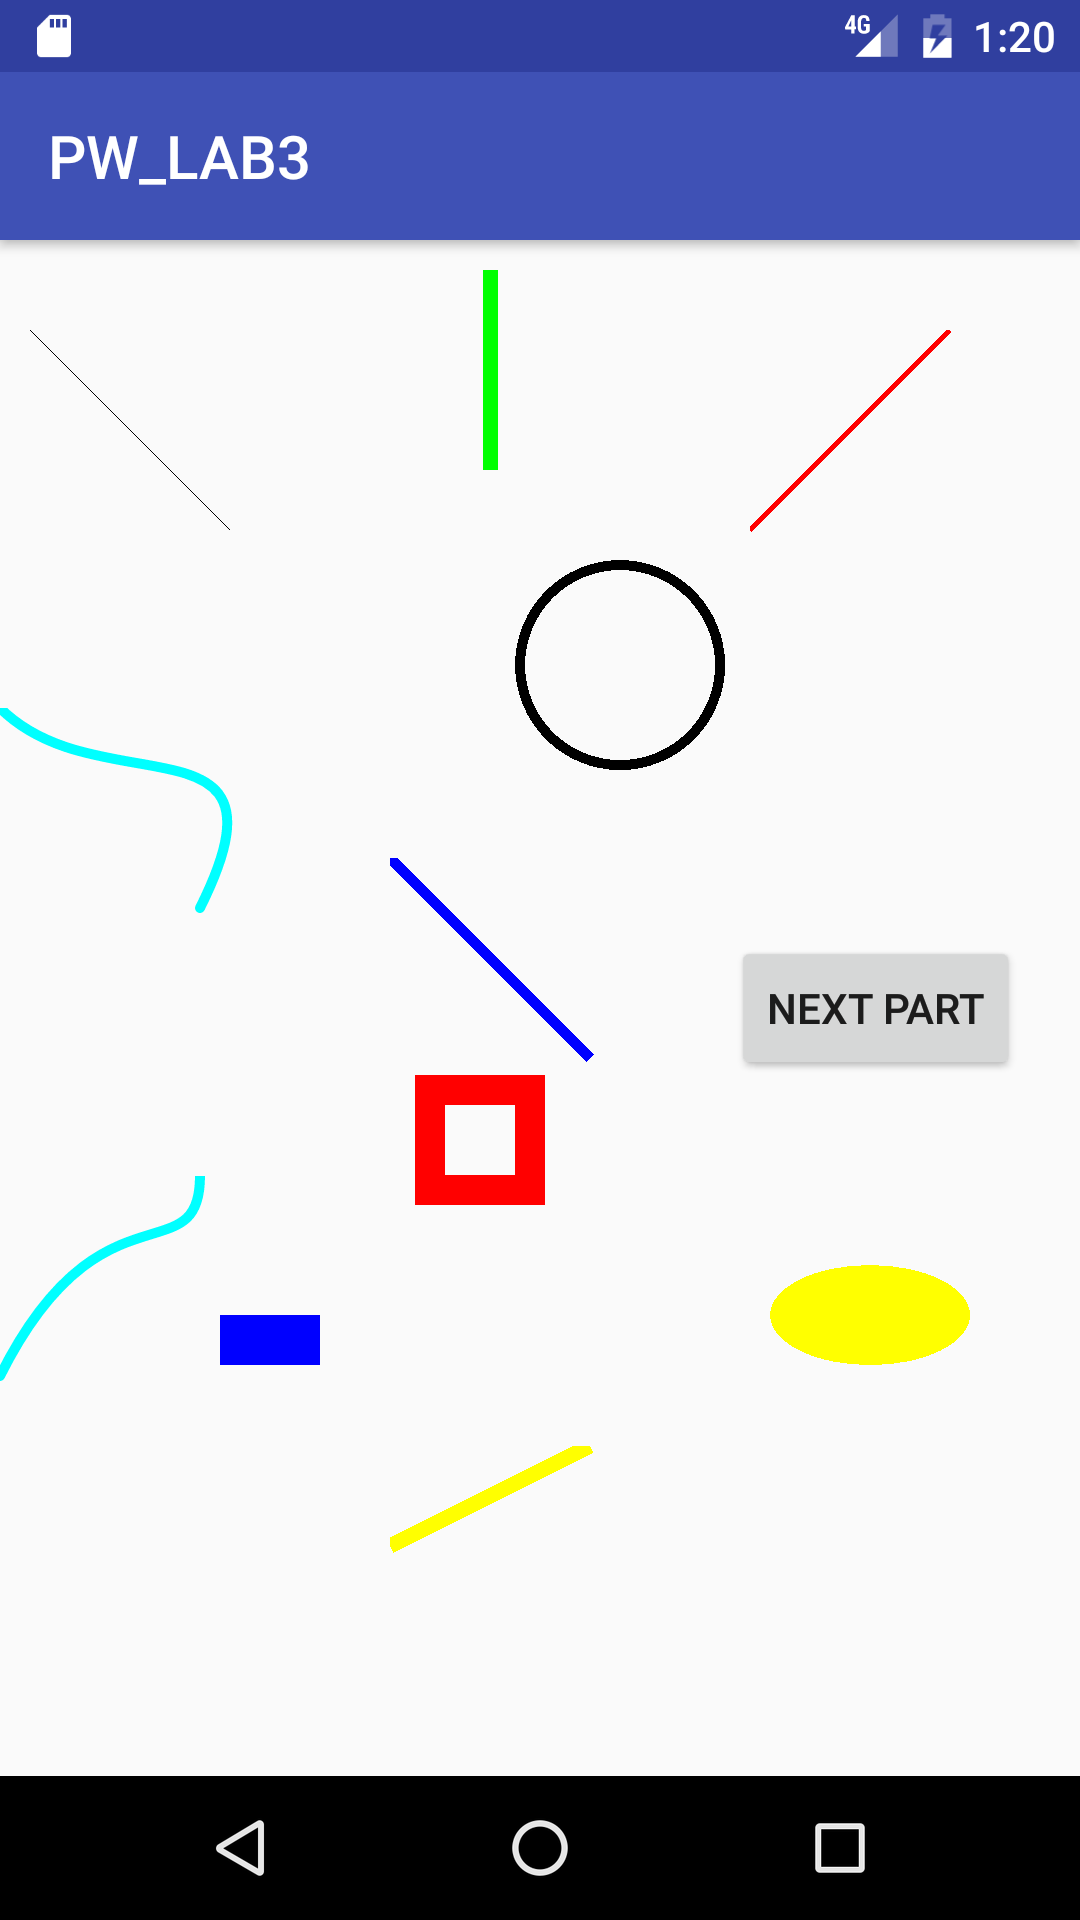
\includegraphics[scale=0.2]{screen1}
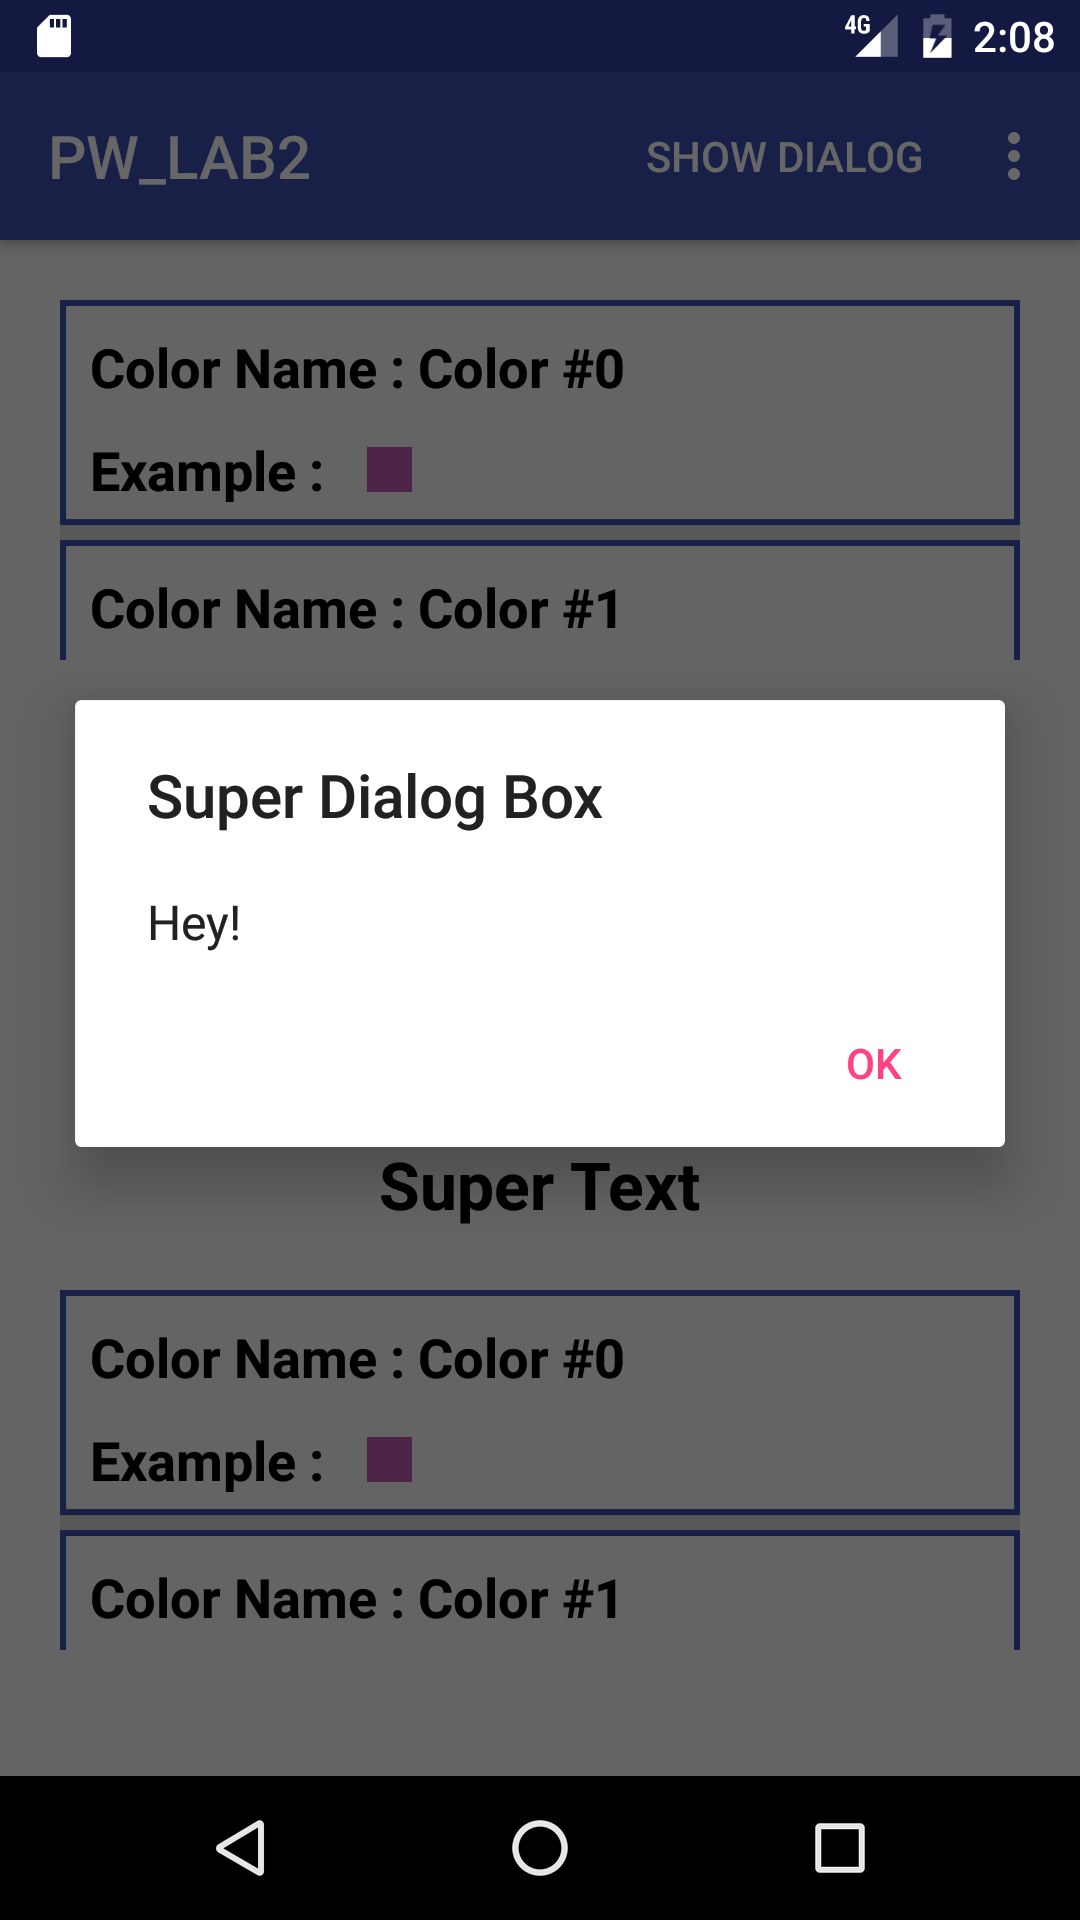
\includegraphics[scale=0.2]{screen2}

b)

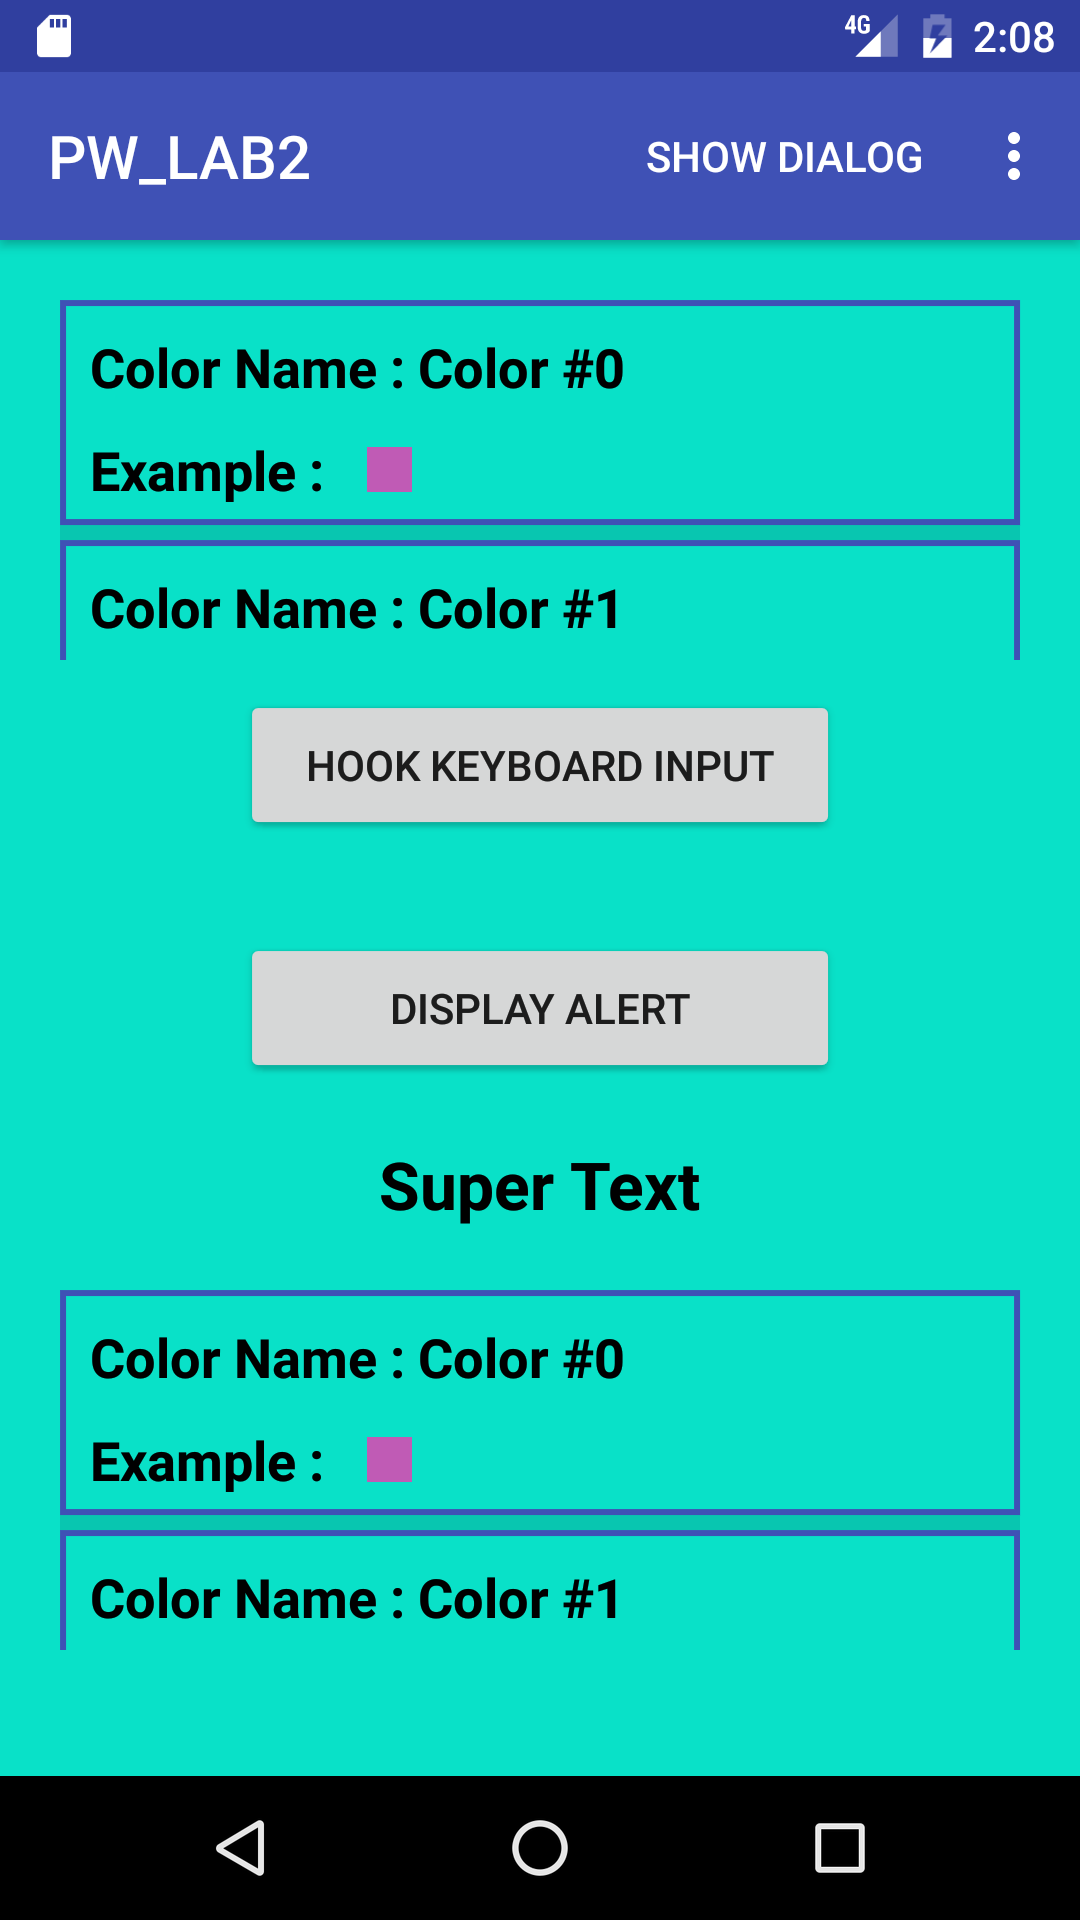
\includegraphics[scale=0.2]{screen3}
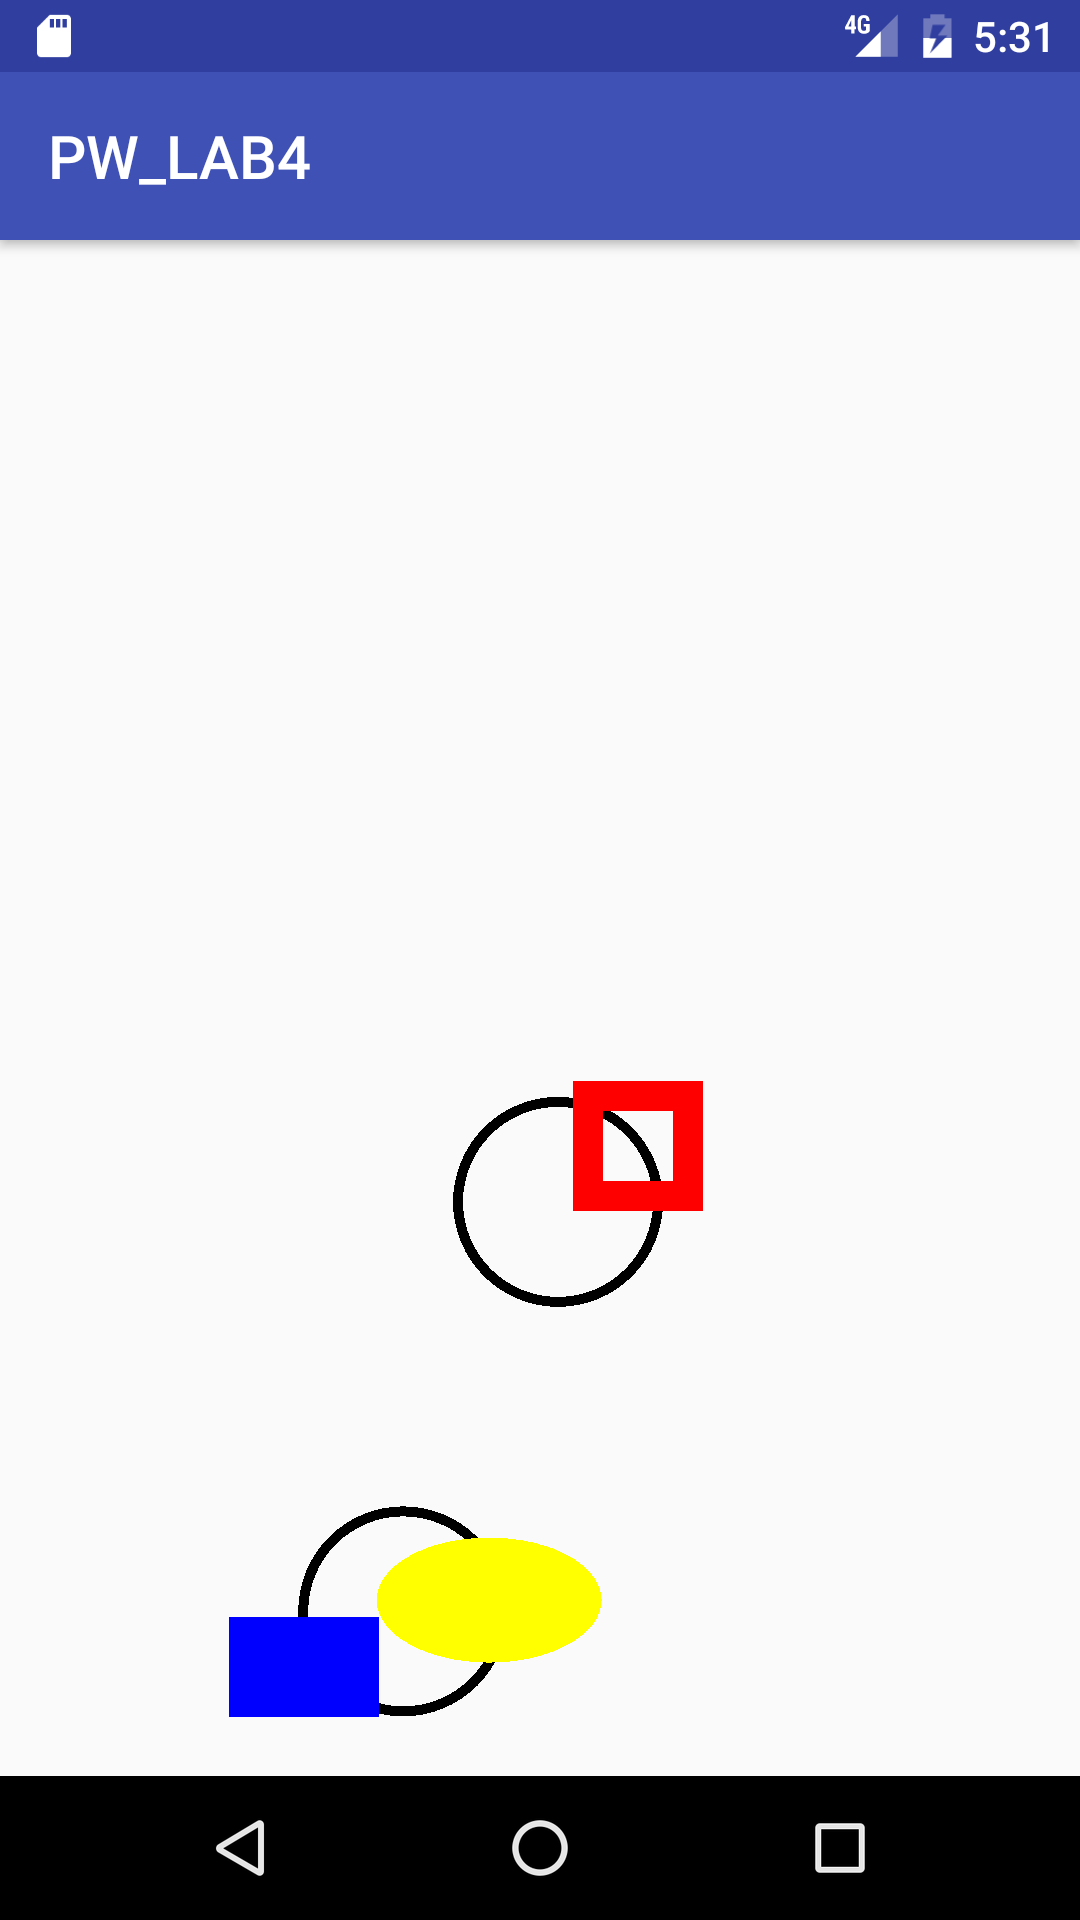
\includegraphics[scale=0.2]{screen4}

c)

"S" clicked

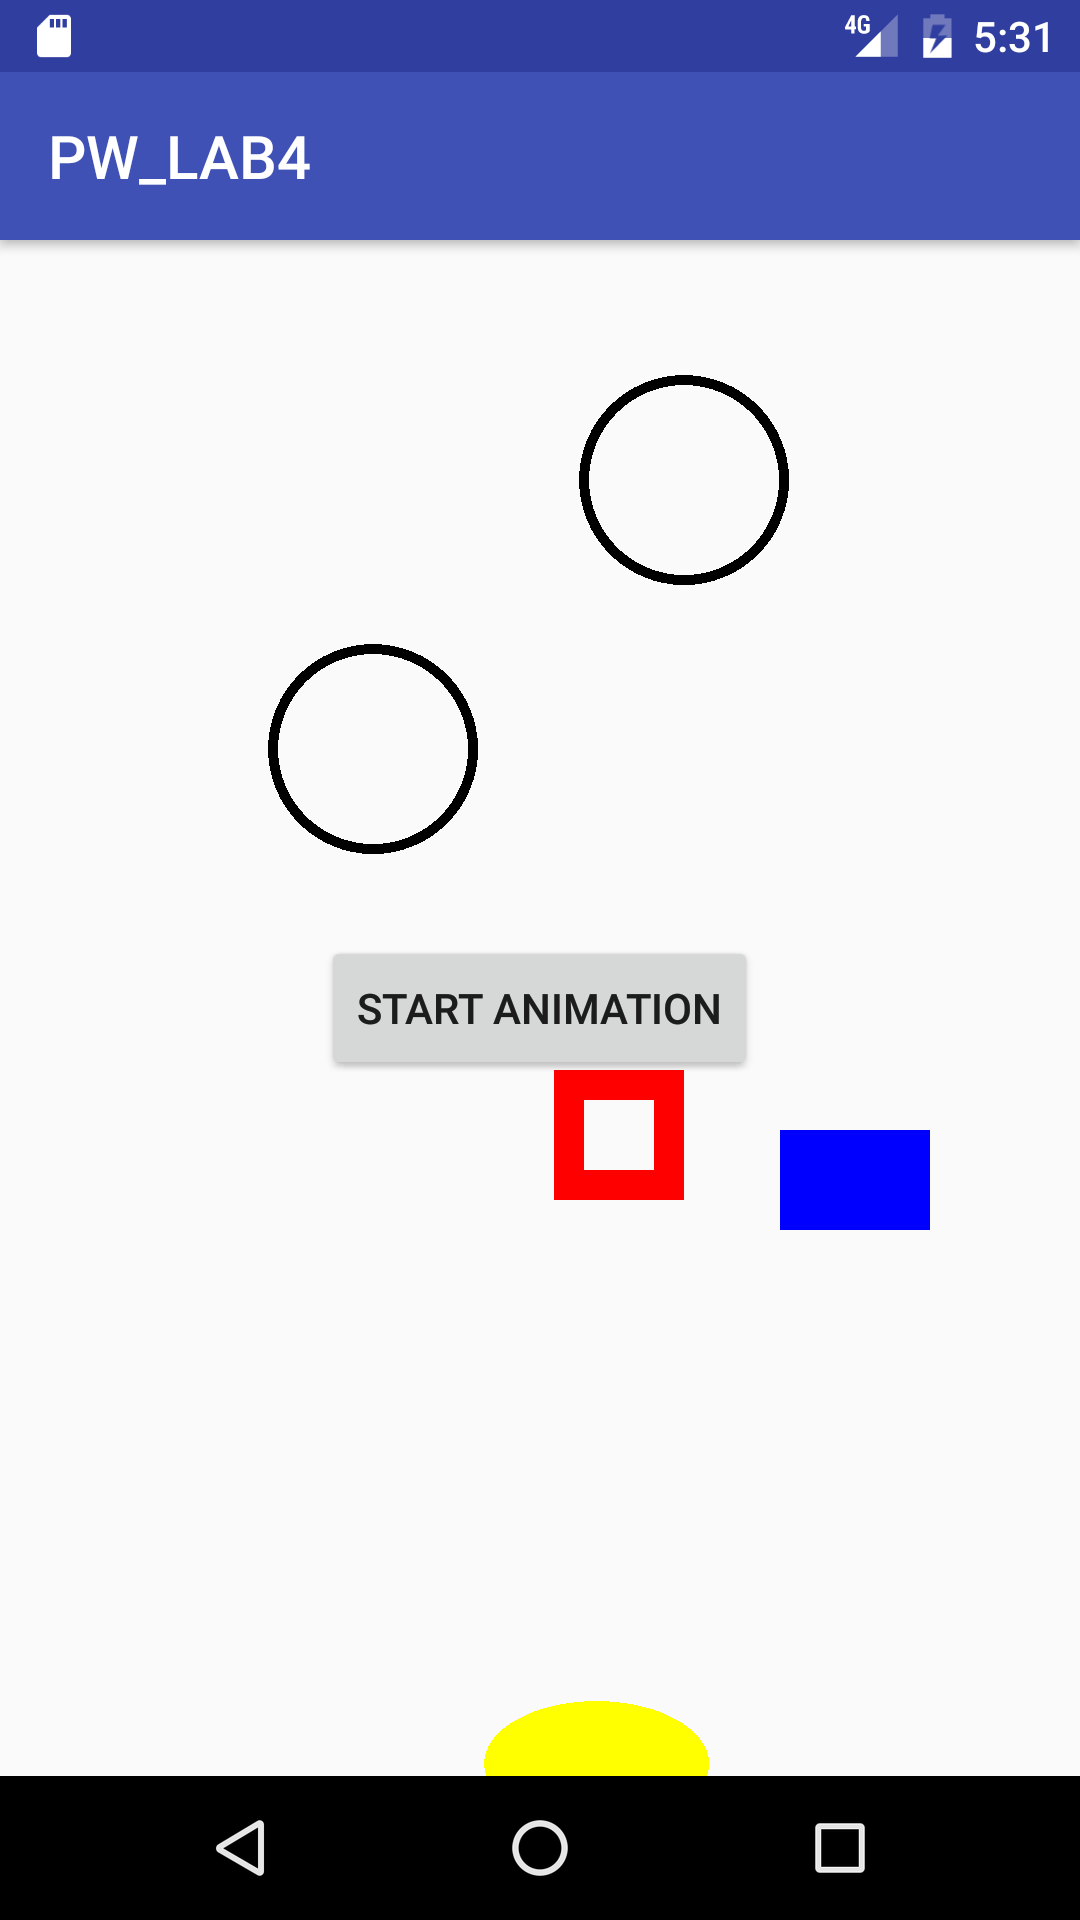
\includegraphics[scale=0.2]{screen5}

"R"clicked 

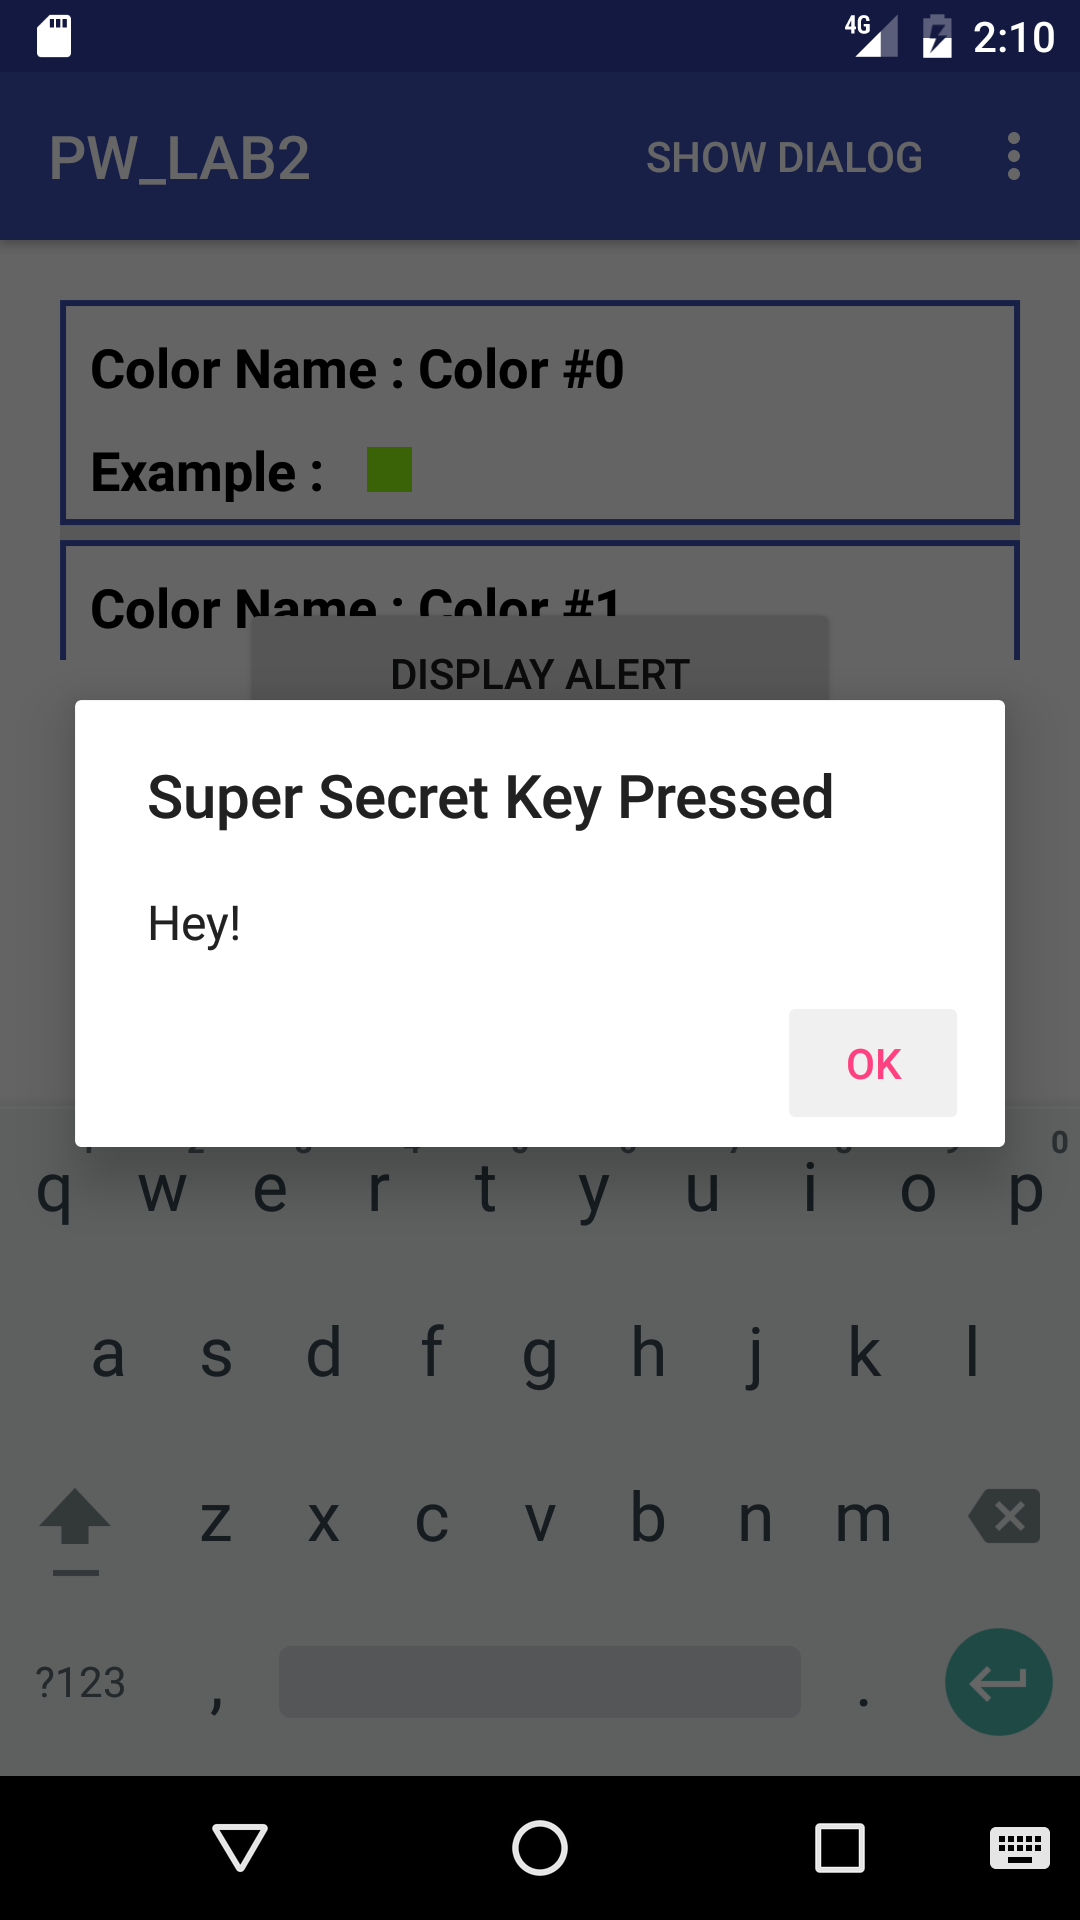
\includegraphics[scale=0.2]{screen6}

d) Top list with scroll bar

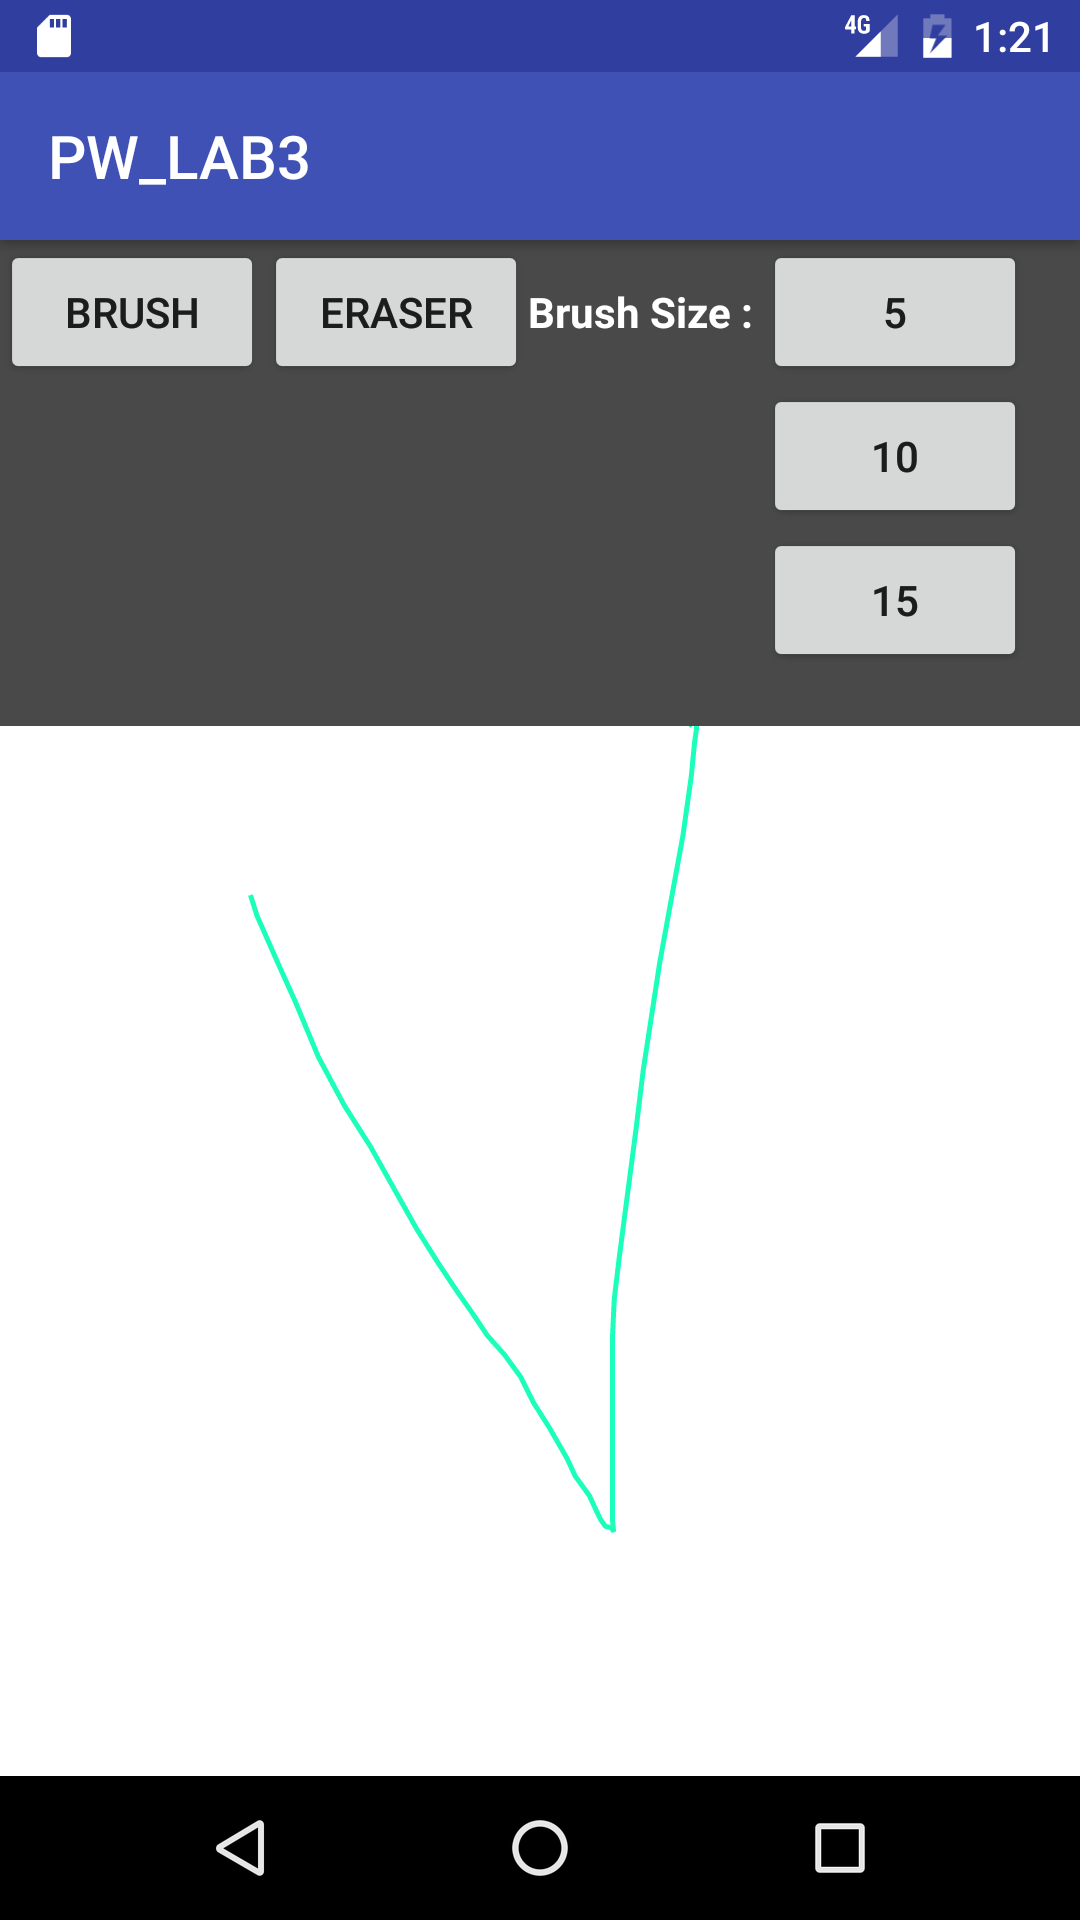
\includegraphics[scale=0.2]{screen7}

e)

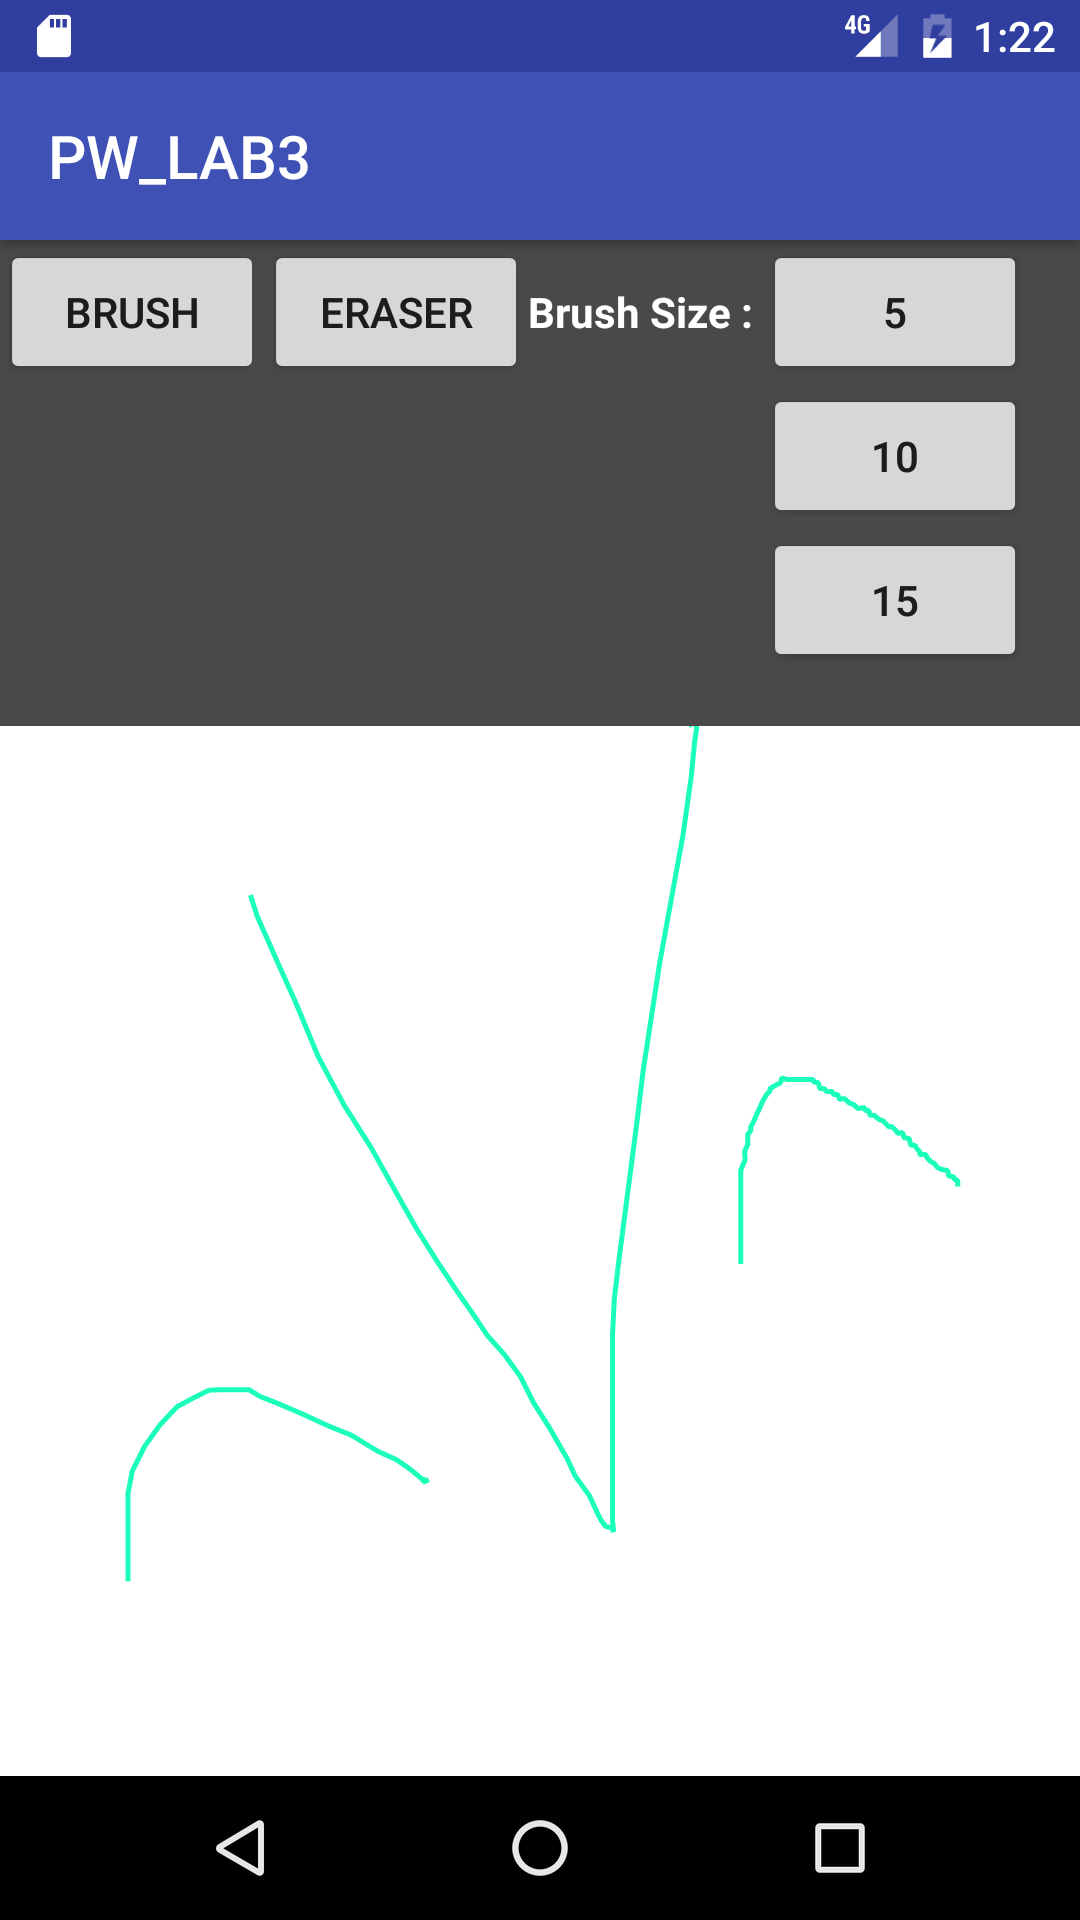
\includegraphics[scale=0.2]{screen8}

f) Bottom list with random action

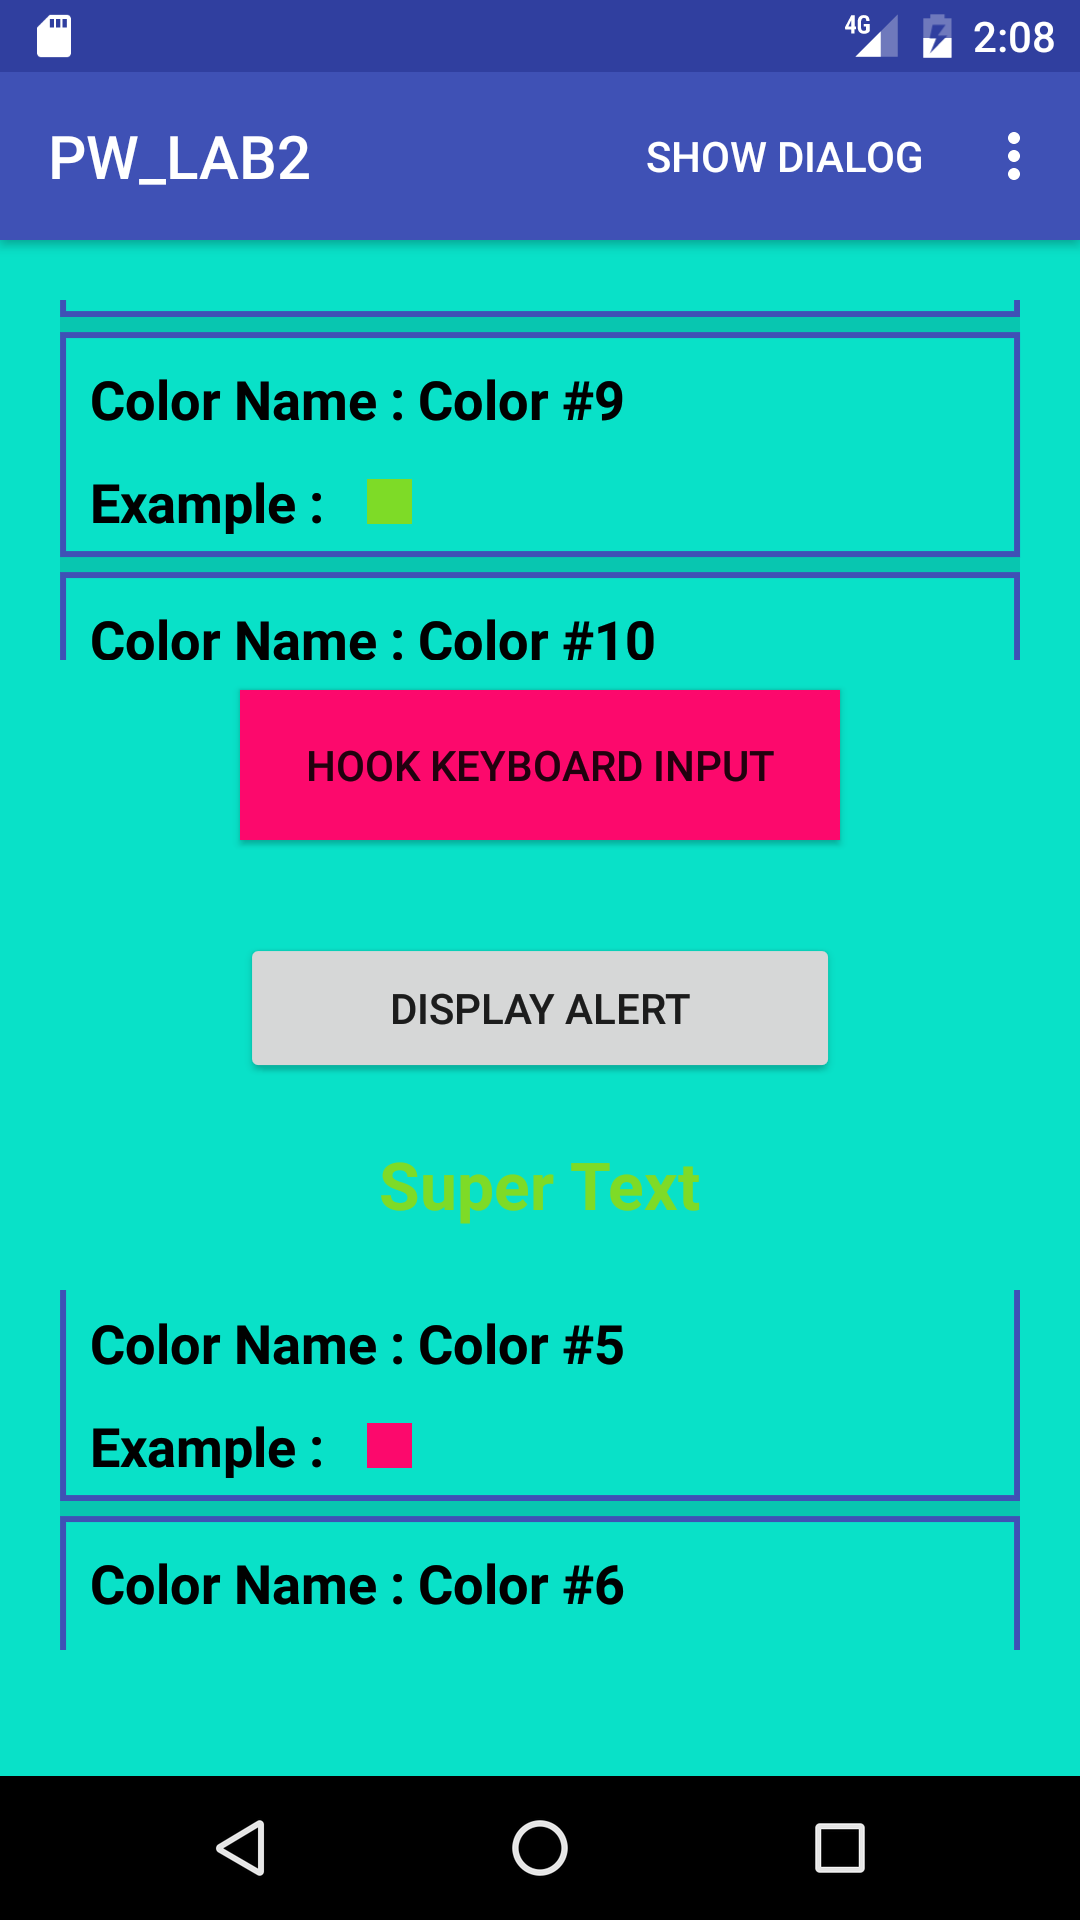
\includegraphics[scale=0.2]{screen9}

\clearpage